\documentclass{article}

\usepackage{graphicx}
\usepackage{gensymb}

\title{AE 1601 Wind Tunnel Activity}
\author{Micaiah Smith-Pierce}
\date{\it{29-March-2017}}

\begin{document}
\maketitle

\section*{Nomenclature}
\begin{tabular}{l l}
b & span \\
c & chord \\
t/c & thickness to chord ratio \\
AR & aspect ratio \\
S & planform area \\
$\alpha$ or AOA & Angle of Attack \\
$C_l$ & Lift Coefficient \\
${C_d}_i$ & Induced Drag Coefficient \\
a & lift curve slope of the (finite) wing \\
$a_0$ & lift curve slope of the airfoil \\
\end{tabular}

\section*{Data Reduction}

\subsection*{Results}
\begin{tabular}{l l l}
v (m/s) & Re & $\alpha_0$ (1/rad)\\ \hline
4 & 3.076957e+04 & 9.596064\\
8 & 6.153914e+04 & 5.413088\\
12 & 9.230871e+04 & 5.590212\\
16 & 1.230783e+05 & 5.762940\\
\end{tabular}

\subsection*{Plotting}
\begin{minipage}{0.5\linewidth}
	\centering
	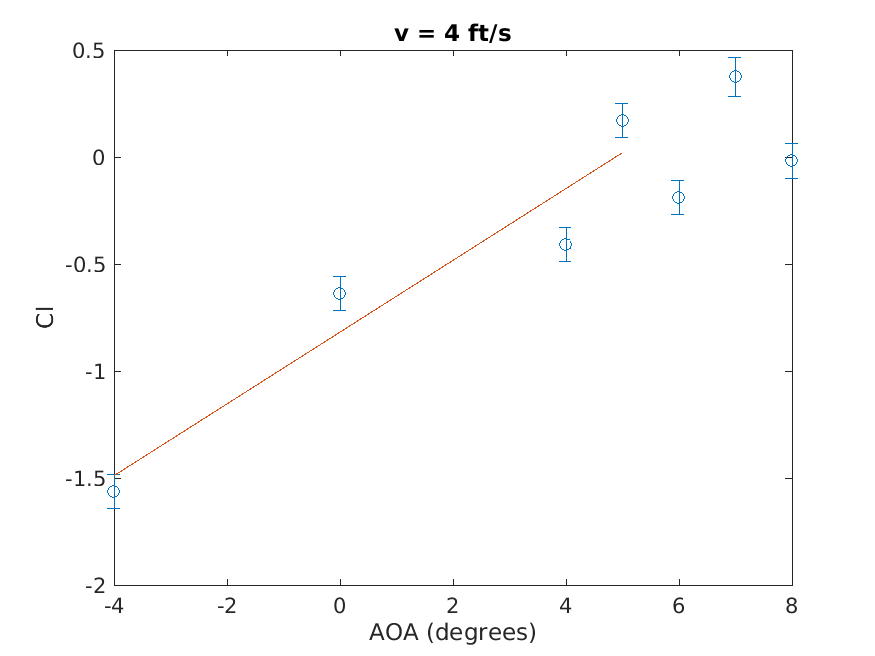
\includegraphics[width = \textwidth]{4plot.png}
\end{minipage}
\begin{minipage}{0.5\linewidth}
	\centering
	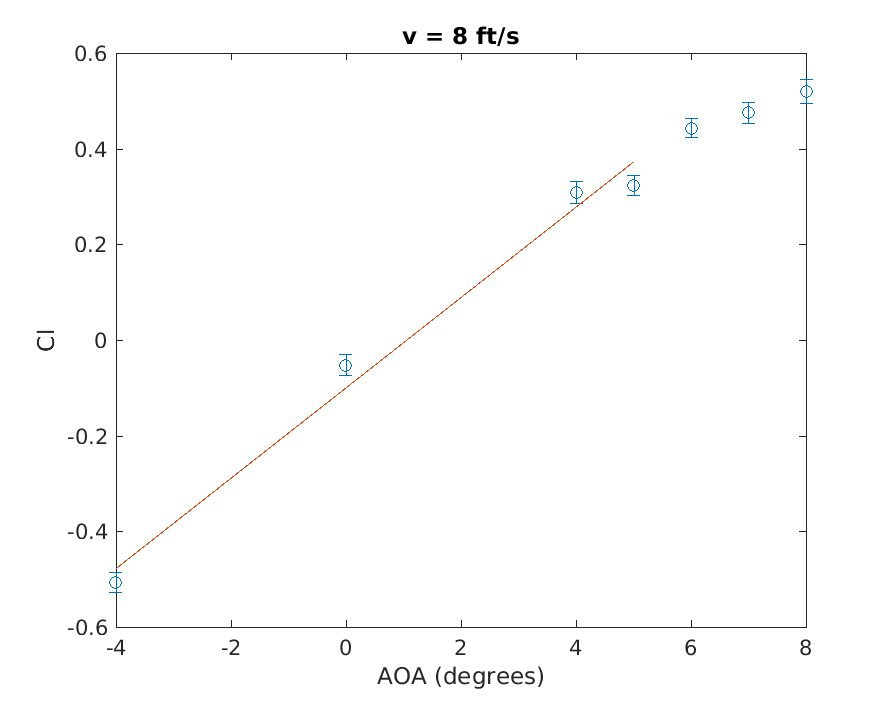
\includegraphics[width = \textwidth]{8plot.png}
\end{minipage}
\begin{minipage}{0.5\linewidth}
	\centering
	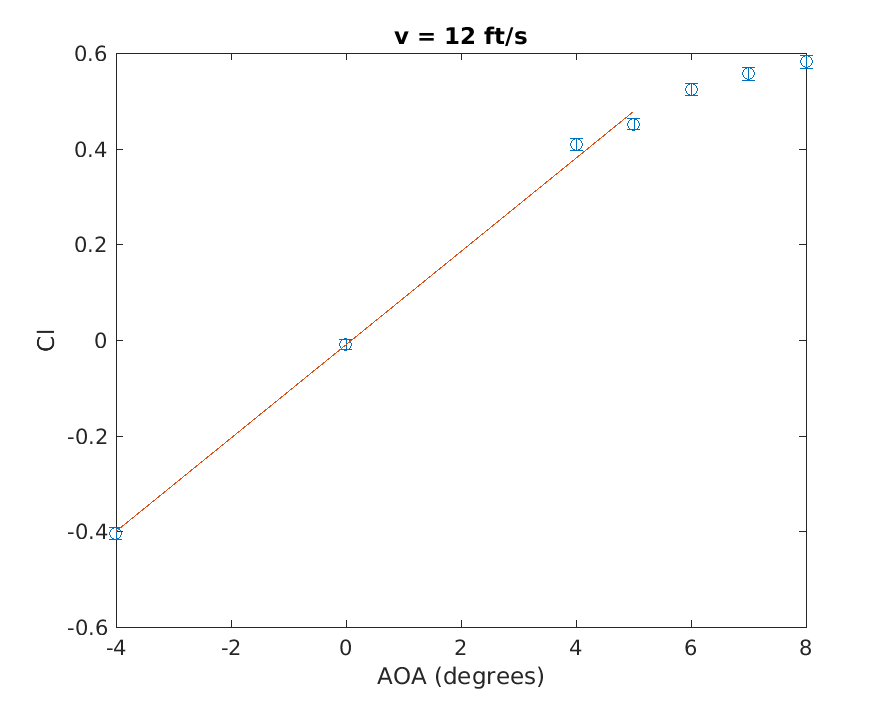
\includegraphics[width = \textwidth]{12plot.png}
\end{minipage}
\begin{minipage}{0.5\linewidth}
	\centering
	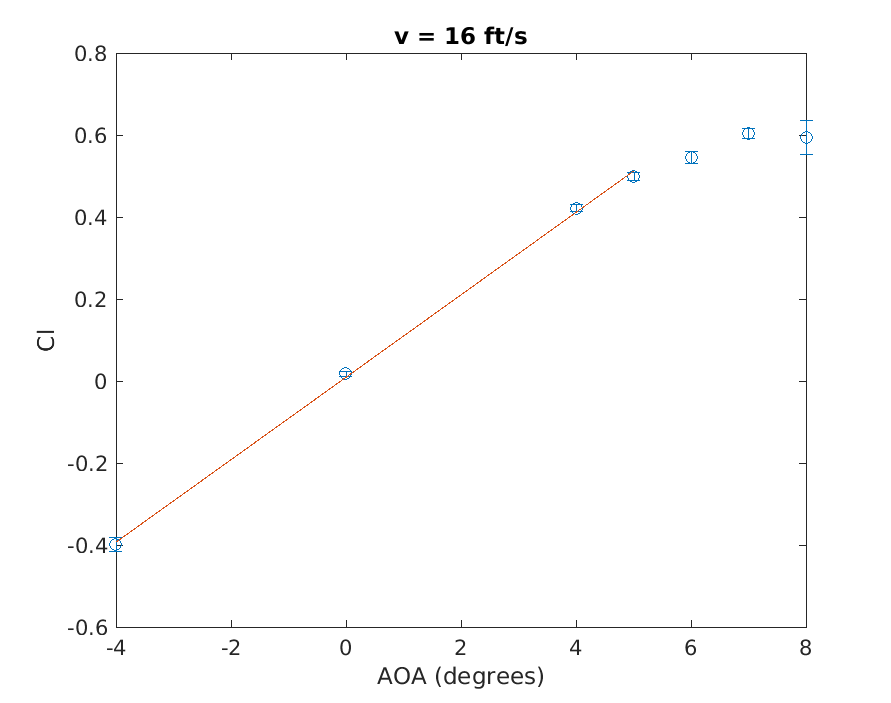
\includegraphics[width = \textwidth]{16plot.png}
\end{minipage}

\section*{Answers to Problems}
\begin{enumerate}

\item Other Group Members:
\begin{itemize}
\item Austin Rose
\item Afiq Manap
\item Meric Taneri
\item Tyler Fuhrman
\item Yohannes Kasseya
\end{itemize}

\item Geometry:

\begin{tabular}{l   l}
b & 0.47m \\
c & 0.12m \\
t/c & 0.42 \\
AR & 3.92 \\
S & $0.06123 m^2$ \\
\end{tabular}

N.B. $S \neq bc$ because the span and area are measurements estimates obtained by treating
the blade as a rectangle.  This inconsistency leads to some ambiguity as to the meaning of
the geometric parameters (i.e. does c refer to 0.12m, or S/b?).  All following calculations
were done using the listed value of each parameter, not any other values that could be obtained
by interpolating between other parameters.  Also, the value of AR was computed as b/c not $b^2 / S$.

\item As I had an excused absence that day, I was unable to take a photograph.

\item Our data:

\begin{tabular}{|l | l | l | l |}
\hline
$\rho (slug/ft^3)$ & Speed (ft/s) & $\alpha$ & Lift (lbf) \\ \hline
2.264353e-03 & 13.12 & $6\degree$ & 0.048 \\ \hline
2.264353e-03 & 26.24 & $6\degree$ & 0.244 \\ \hline
2.264353e-03 & 39.36 & $6\degree$ & 0.644 \\ \hline
2.264353e-03 & 52.49 & $6\degree$ & 1.242 \\ \hline
\end{tabular}

\begin{tabular}{|l | l | l | l |}
\hline
$\rho (kg/m^3)$ & Speed (m/s) & $\alpha$ & Lift (N) \\ \hline
1.167 & 4 & $6\degree$ & 0.213 \\ \hline
1.167 & 8 & $6\degree$ & 1.087 \\ \hline
1.167 & 12 & $6\degree$ & 2.866 \\ \hline
1.167 & 16 & $6\degree$ & 5.525 \\ \hline
\end{tabular}

\item It appears Professor Komerath expected each group to perform measurements at a range of $\alpha$ values.
The activity was conducted such that each group took measurements at only one $\alpha$ value, at a range of
velocities.  Nevertheless, we have the degenerate table:

\begin{tabular}{c | c}
$\alpha$ & $C_l$ \\ \hline
$6\degree$ & 0.330 \\
\end{tabular}

\item The data, agregated over velocities, is tabulated below.

\begin{tabular}{c | c}
$\alpha$ & $C_l$ \\ \hline
$-4\degree$ & -0.718 \\ \hline 
$0\degree$ & -0.171 \\ \hline 
$4\degree$ & 0.182 \\ \hline 
$5\degree$ & 0.360 \\ \hline 
$6\degree$ & 0.330 \\ \hline 
$7\degree$ & 0.502 \\ \hline 
$8\degree$ & 0.419 \\
\end{tabular}

\item The aggregated data is plotted below:

\begin{minipage}{0.5\linewidth}
	\centering
	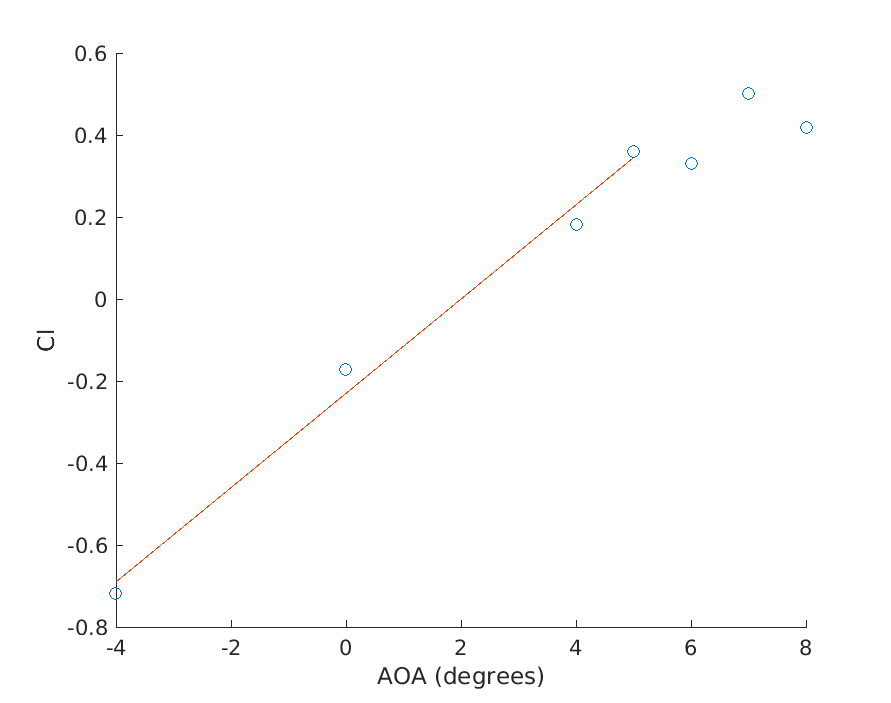
\includegraphics[width = 0.99\textwidth]{cl.png}
\end{minipage}
\begin{minipage}{0.5\linewidth}
	\centering
	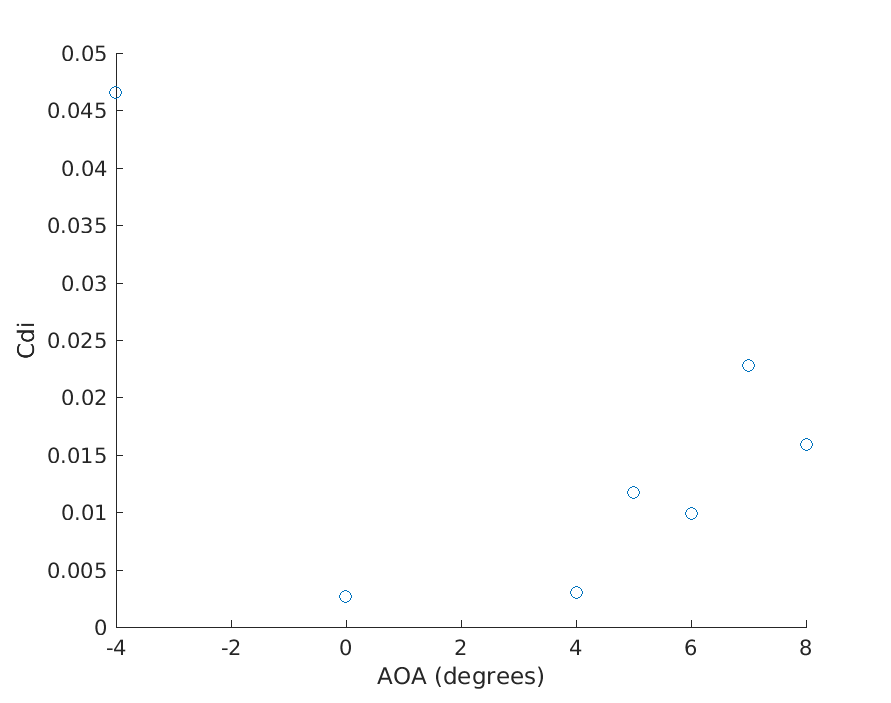
\includegraphics[width = 0.99\textwidth]{cdi.png}
\end{minipage}

\item The slope of the linear fit was calculated using MATLAB's \verb|polyfit| function.  The value is 6.59/rad.  Using the formula
\[a_0 = \frac{a}{1 - \frac{a e}{\pi AR}}\]
$a_0$ was calculated to be 6.65/rad.

\end{enumerate}
\end{document}
